Visual odometry\cite{he_tvc2019} and \gls{feature}-based localization with optical sensors\cite{sattler_cvpr2018} are established technologies in robotics.
Additionally, the use of depth sensors increased with their availability and fast integration into robotic systems.
This naturally leads to the task of exploiting the depth information for problems like localization and mapping, which at their core require to align multiple pointclouds to each other.
One dominant algorithm to solve this problem is \acrshort{icp} (\acrlong{icp})\cite{besl_pami1992}.
It has various characteristics and limitations that require an initial estimate for the relative pose between pointclouds\cite{rusinkiewicz_ieee2001}.
Loop closure in \acrshort{slam} (\acrlong{slam})\cite{ho_ros2006}, global localization and place recognition\cite{sattler_2011} can not rely on such an initial estimate.
Those problems are commonly solved with a \gls{feature}-based approach, that detects distinctive points in different color images and finds correspondences of real world elements captured from multiple views.
Detecting salient points in an image and describing the local neighbourhood in a recognizable manner is at the core of many solutions of computer vision related problems and a well researched topic\cite{andersson_2016}.

The aim of this thesis is to transfer this technology from optical images to depth images and range data from \acrshort{LIDAR} scans by proposing the novel \Gls{flexion-image}.
Visual features require local brightness gradients that are not present in raw depth images.
Therefore, a conversion of the depth image to a derived image encodes local geometrical relationships of neighbouring depth pixels and results in an image that feature detectors can work on --- a feature image.
Standard feature detectors and descriptors, namely \acrshort{sift}, \acrshort{surf}, \acrshort{orb} and \acrshort{akaze}, can then detect interesting geometrical shapes as normal keypoints.
Their surroundings and real world context are captured with the keypoint descriptor.
Scale and orientation detection are part of the keypoint detector.
\begin{figure}[htb]
    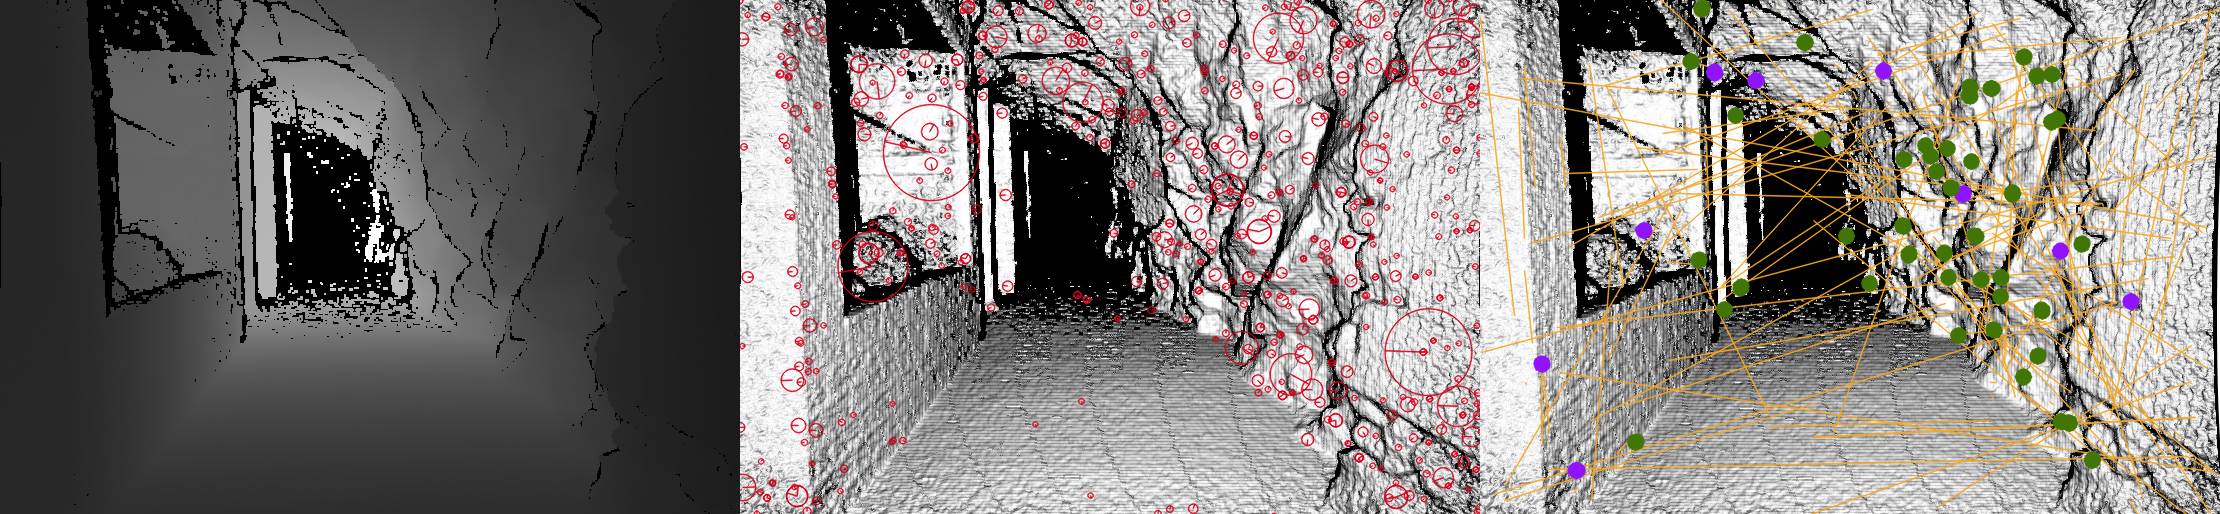
\includegraphics[width=\linewidth]{chapter01/masterarbeit_method.png}
    \caption[Illustration of Feature Detection and Matching on \Glspl{flexion-image}]{\emph{Illustration of Feature Detection and Matching on \Glspl{flexion-image}.} This figure demonstrates the processing steps from depth image (left) to features detected on a converted \gls{flexion-image} (middle) that are matched between multiple views (right). Green points indicate correctly identified correspondences between consecutive images, undetected correspondences are purple and orange lines indicate incorrect matches.}\label{fig:method_example}
\end{figure}

The proposed feature images have different visual characteristics than color images.
A \gls{feature}-based depth data registration requires stable keypoints between multiple views and a discriminating descriptor between different geometries (Figure~\ref{fig:method_example}).
Researching the properties of both the keypoints and the descriptors is therefore mandatory work before solving more complex tasks like global localization.
This work is part of developing robotic systems for underground mining environments.
It is common to have detailed \acrshort{LIDAR} scans of mine segments, which is a part of mine surveying.
Bad lighting conditions challenge the classical optical systems and algorithms.
Other techniques, like GPS, are outright impossible to use.
A positive outcome of the proposed method can be the first step towards using \acrshort{LIDAR} scans as map.

The main contribution of this thesis is a novel way to convert depth data into a derived feature image and the in-depth analysis of the performance of keypoint detectors and descriptors on feature images.
All developed tools can be reused as both library code and executable binary to create such images and run \gls{feature} algorithms on them.
Both the qualitative and quantitative findings build an empirical foundation on developing this approach further for more complex feature-based tasks.

Section~\ref{sec:related_work} introduces the related work on pointcloud registration and \gls{feature} performance comparisons.
Necessary foundational knowledge on depth sensors and the math of modeling their data is presented in Section~\ref{sec:fundamentals}.
Additionally, it gives a high level introduction on keypoint detectors and descriptors and how their performance can be evaluated.
Section~\ref{sec:image_processing} describes the novel depth data processing pipeline, starting with edge-preserving filtering followed by conversion to feature images and finally explaining the evaluated \gls{feature} detection and description algorithms.
The experiments evaluate this process.
Section~\ref{sec:experiments} describes the metrics, datasets and algorithm configurations.
Section~\ref{sec:results} presents and discusses the results.
Finally, Section~\ref{sec:conclusion} concludes the work and proposes further research areas.
